% !TEX TS-program = pdflatex
% !TEX encoding = UTF-8 Unicode

\documentclass[12pt]{article} 

\usepackage[utf8]{inputenc} % set input encoding 

\usepackage{geometry} % to change the page dimensions
\geometry{a4paper} 
\usepackage[parfill]{parskip} % No indent in document

% Packages
\usepackage{graphicx}
\usepackage{array}
\usepackage{amsmath}
\usepackage{amssymb}
\usepackage{verbatim}
\usepackage{xcolor}
\usepackage[hidelinks]{hyperref}
\usepackage{todonotes}
\usepackage{tikz}
\usepackage{multicol}

%\renewcommand{\arraystretch}{1.2}

% Define colors
\definecolor{mint}{rgb}{0.65,0.84,0.82}
\definecolor{scheme}{rgb}{0,0,1}

\title{Bitcoin, Blockchain and Cryptoassets \\ Solutions Exercise Set 1}
\author{}
\date{ } 

\begin{document}
\maketitle

\newpage

\section*{Exercise 1}
\label{sec:numeralSystems}
This first exercise looked at the conversion between different numeral systems.
\subsection*{Exercise 1.1}

\begin{itemize}
	\item[a)] Convert the binary number $({\tt10110101})_{B=2}$ into a decimal number.
	\vspace{0.5cm}
	\begin{figure}[h!]
		\centering
		\resizebox{10cm}{2.045cm}{ % {width}{hight}
			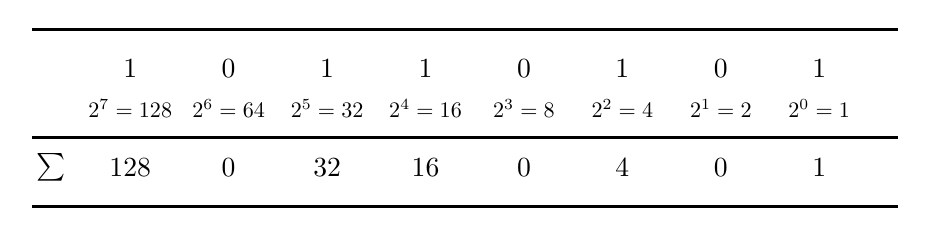
\begin{tikzpicture}[domain=0:11]
				\draw[very thick] (0,0) -- (11,0);
				\draw[very thick] (0,2.25) -- (11,2.25);
				\draw[thick] (0,.875) --(11,.875); 
				
					\draw (10,1.75) node {$1$};
					\draw (8.75,1.75) node {$0$};
					\draw (7.5,1.75) node {$1$};
					\draw (6.25,1.75) node {$0$};
					\draw (5,1.75) node {$1$};
					\draw (3.75,1.75) node {$1$};
					\draw (2.5,1.75) node {$0$};
					\draw (1.25,1.75) node {$1$};
				
					\draw (10,1.25) node [scale = 0.8] {$2^{0}=1$};
					\draw (8.75,1.25) node [scale = 0.8] {$2^{1}=2$};
					\draw (7.5,1.25) node [scale = 0.8] {$2^{2}=4$};
					\draw (6.25,1.25) node [scale = 0.8] {$2^{3}=8$};
					\draw (5,1.25) node [scale = 0.8] {$2^{4}=16$};
					\draw (3.75,1.25) node [scale = 0.8] {$2^{5}=32$};
					\draw (2.5,1.25) node [scale = 0.8] {$2^{6}=64$};
					\draw (1.25,1.25) node [scale = 0.8] {$2^{7}=128$};

					\draw (10,.5) node {$1$};
					\draw (8.75,.5) node {$0$};
					\draw (7.5,.5) node {$4$};
					\draw (6.25,.5) node {$0$};
					\draw (5,.5) node {$16$};
					\draw (3.75,.5) node {$32$};
					\draw (2.5,.5) node {$0$};
					\draw (1.25,.5) node {$128$};

					\draw (.25,.5) node {$\sum$};
			\end{tikzpicture}
		}
	\end{figure}

	$\rightarrow \quad \sum = 181 \quad \rightarrow \quad (10110101)_{B=2} = (181)_{B=10}$
	\vspace{0.2cm}

	\item[b)] Conver the decimal number $(93)_{B = 10}$ into a binary number.
	
	\begin{figure}[h!]
		\centering
		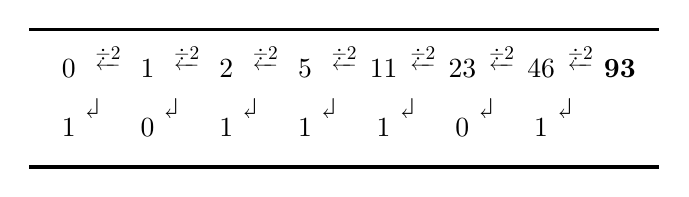
\begin{tikzpicture}
			\draw[very thick] (0,0) -- (8,0);
			\draw[very thick] (0,1.75) -- (8,1.75);
			\draw (7.5,1.25) node {$\textbf{93}$};

				\draw (6.5,1.25) node {$46$};
				\draw (7,1.38) node[scale = 0.7] {$\underleftarrow{\div 2}$};
				\draw (6.5,.5) node {$1$};
				\draw (6.8,.75) node {$\rotatebox[origin=c]{180}{$\Rsh$} $};

				\draw (5.5,1.25) node {$23$};
				\draw (6,1.38) node[scale = 0.7] {$\underleftarrow{\div 2}$};
				\draw (5.5,.5) node {$0$};
				\draw (5.8,.75) node {$\rotatebox[origin=c]{180}{$\Rsh$} $};

				\draw (4.5,1.25) node {$11$};
				\draw (5,1.38) node[scale = 0.7] {$\underleftarrow{\div 2}$};
				\draw (4.5,.5) node {$1$};
				\draw (4.8,.75) node {$\rotatebox[origin=c]{180}{$\Rsh$} $};

				\draw (3.5,1.25) node {$5$};
				\draw (4,1.38) node[scale = 0.7] {$\underleftarrow{\div 2}$};
				\draw (3.5,.5) node {$1$};
				\draw (3.8,.75) node {$\rotatebox[origin=c]{180}{$\Rsh$} $};

				\draw (2.5,1.25) node {$2$};
				\draw (3,1.38) node[scale = 0.7] {$\underleftarrow{\div 2}$};
				\draw (2.5,.5) node {$1$};
				\draw (2.8,.75) node {$\rotatebox[origin=c]{180}{$\Rsh$} $};

				\draw (1.5,1.25) node {$1$};
				\draw (2,1.38) node[scale = 0.7] {$\underleftarrow{\div 2}$};
				\draw (1.5,.5) node {$0$};
				\draw (1.8,.75) node {$\rotatebox[origin=c]{180}{$\Rsh$} $};

				\draw (.5,1.25) node {$0$};
				\draw (1,1.38) node[scale = 0.7] {$\underleftarrow{\div 2}$};
				\draw (.5,.5) node {$1$};
				\draw (0.8,.75) node {$\rotatebox[origin=c]{180}{$\Rsh$} $};

		\end{tikzpicture}
	\end{figure}
	$\rightarrow \quad (93)_{B=10} = (01011101)_{B=2}$
\end{itemize}

\subsection*{Exercise 1.2}

\begin{itemize}
	\item[a)] Convert the binary number $({\tt10110101})_{B=2}$ into a hexadecimal.\\
	Each hexadecimal number represents four binary numbers (as $2^{4} = 16$).\\
	
	\begin{figure}[h!]
		\centering
		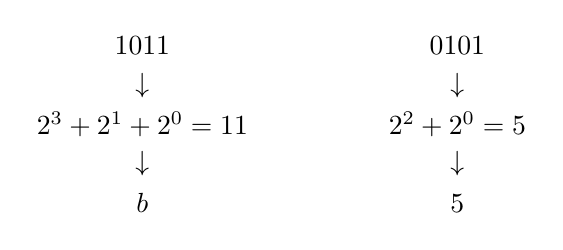
\begin{tikzpicture}
				\draw (7,2) node {$0101$};
				\draw (3,2) node {$1011$};
				\draw (7,1.5) node {$\downarrow$};
				\draw (3,1.5) node {$\downarrow$};
				\draw (7,1) node {$2^{2} + 2^{0} = 5$};
				\draw (3,1) node {$2^{3} + 2^{1} + 2^{0} = 11$};
				\draw (7,.5) node {$\downarrow$};
				\draw (7,0) node {$5$};
				\draw (3,.5) node {$\downarrow$};
				\draw (3,0) node {$b$};
		\end{tikzpicture}
	\end{figure}
	$\rightarrow \quad (10110101)_{B=2} = (b5)_{B=16}$
\end{itemize}
\newpage
\begin{itemize}	
	\item[b)] Convert the hexadecimal $($9c3a$)_{B = 16}$ into a binary number.
	
	\begin{figure}[h!]
		\centering
		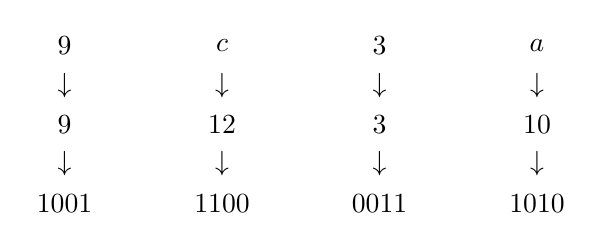
\begin{tikzpicture}
				\draw (2,2) node {$9$};
				\draw (4,2) node {$c$};
				\draw (6,2) node {$3$};
				\draw (8,2) node {$a$};

				\draw (2,1.5) node {$\downarrow$};
				\draw (4,1.5) node {$\downarrow$};
				\draw (6,1.5) node {$\downarrow$};
				\draw (8,1.5) node {$\downarrow$};
				
				\draw (2,1) node {$9$};
				\draw (4,1) node {$12$};
				\draw (6,1) node {$3$};
				\draw (8,1) node {$10$};

				\draw (2,.5) node {$\downarrow$};
				\draw (4,.5) node {$\downarrow$};
				\draw (6,.5) node {$\downarrow$};
				\draw (8,.5) node {$\downarrow$};
				
				\draw (2,0) node {$1001$};
				\draw (4,0) node {$1100$};
				\draw (6,0) node {$0011$};
				\draw (8,0) node {$1010$};
		\end{tikzpicture}
	\end{figure}
	$\rightarrow \quad$ (9c3a)$_{B=16} = (1001110000111010)_{B=2}$
\end{itemize}

\newpage


\section*{Exercise 2}
\label{sec:monoalphabetic}
The following encrypted (English) text was given in the exercise:\par

RQL IFMXAXQKNY XQKFFLYZL NH K ZJLKR MOOMJRGYNRD RM ZKNY OJKXRNXKF LPOLJNLYXL TGJNYZ DMGJ HRGTNLH KYT RM UMJA MY K FKJZLJ OJMVLXR RMZLRQLJ UNRQ K XMEOKYD.\\
RQL HRGTLYR RLKEH TLHNZY K HMFGRNMY MY RQL IKHNH MC K OJKXRNXL-MJNLYRLT OJMIFLE TLHXJNORNMY. KXXMEOKYNLT ID XMKXQLH KYT LPOLJRH, RQLD ZM RQJMGZQ RQL HRLOH NY XJLKRNYZ K XMYXLOR NYXFGTNYZ K OJMRMRDOL. RQNH KNEH KR HRJLYZRQLYNYZ RQLNJ RLKEUMJA, MJZKYNHKRNMYKF KYT OJLHLYRKRNMY HANFFH, KH ULFF KH NEOJMWNYZ RNEL EKYKZLELYR KYT OJMIFLE-HMFWNYZ XMEOLRLYXL. CGJRQLJEMJL, RQL XQKFFLYZL MCCLJH K GYNBGL XQKYXL RM YLRUMJA UNRQ XMEOKYNLH KYT LPOLJRH KH ULFF KH HRGTLYRH UQM KJL NYRLJLHRLT NY RQL HKEL RMONXH.\par

By counting the occurances of the letters (or using the referenced online tool) one arrives at the following table showing the relative frequencies of the letters:

\begin{table}[h!]
	\centering
	\resizebox{\textwidth}{!} {
	\begin{tabular}{c c c c c c c c c c }
		\multicolumn{4}{c}{Text} && & \multicolumn{4}{c}{English Language}\\
		\cline{1-4} \cline{7-10}
		&&&&&&&&&\\[-3.3mm]
		Letter & Frequency (\%) & Letter & Frequency (\%) &&& Letter & Frequency (\%) & Letter & Frequency (\%)\\ [1mm]
		\cline{1-4} \cline{7-10}
		&&&&&&&&&\\[-3.5mm]
		A & 0.9 & N & 7.2&&&a & \textcolor{magenta}{8.04} & n & 7.23\\
		B & 0.2 & O & 4.1&&&b & 1.48 & o & 7.64\\
		C & 0.7 & P & 0.6&&&c & 3.34 & p & 2.14\\
		D & 1.1 & Q & 4.1&&&d & 3.82 & q & 0.12\\
		E & 2.8 & R & \textcolor{teal}{9.9}&&&e & \textcolor{blue}{12.49} & r & 6.28\\
		F & 3.5 & S & 0.0&&&f & 2.40 & s & 6.51\\
		G & 2.2 & T & 2.8&&&g & 1.87 & t & \textcolor{teal}{9.28}\\
		H & 6.3 & U & 1.5&&&h & 5.05 & u & 2.73\\
		I & 0.9 & V & 0.2&&&i & 7.57 & v & 1.05\\
		J & 6.3 & W & 0.4&&&j & 0.16 & w & 1.68\\
		K & \textcolor{magenta}{8.5} & X & 4.8&&&k & 0.54 & x & 0.23\\
		L & \textcolor{blue}{12.3} & Y & 8.3&&&l & 4.07 & y & 1.66\\
		M & 7.4 & Z & 3.3&&&m & 2.51 & z & 0.09\\
		\cline{1-4} \cline{7-10}
\end{tabular}}
\caption{Frequencies of letters in the text (left) and in the \href{http://norvig.com/mayzner.html}{English language} (right)}
\end{table}

When replacing the three most frequent letters in the text with the three most frequent letters in the english alphabet we receive the following partially decrypted text. Note that as in the lecture, capital letters stand for encrypted and small letters for plain text letters.
\newpage
tQe IFMXAXQaNY XQaFFeYZe NH a ZJeat MOOMJtGYNtD tM ZaNY OJaXt-\\NXaF ePOeJNeYXe TGJNYZ DMGJ HtGTNeH aYT tM UMJA MY a FaJZeJ OJMVeXt tMZetQeJ UNtQ a XMEOaYD.\\
tQe HtGTeYt teaEH TeHNZY a HMFGtNMY MY tQe IaHNH MC a OJaXtNXe-MJNeYteT OJMIFeE TeHXJNOtNMY. aXXMEOaYNeT ID XMaXQeH aYT ePOeJtH, tQeD ZM tQJMGZQ tQe HteOH NY XJeatNYZ a XMYXeOt NYXFGTNYZ a OJMtMtDOe. tQNH aNEH at HtJeYZtQeYNYZ tQeNJ teaEUMJA, MJZaYNHatNMYaF aYT OJeHeYtatNMY HANFFH, aH UeFF aH NEOJMWNYZ tNEe EaYaZeEeYt aYT OJMIFeE-HMFWNYZ XMEOeteYXe. CGJtQeJEMJe, tQe XQaFFeYZe MCCeJH a GYNBGe XQaYXe tM YetUMJA UNtQ XMEOaYNeH aYT ePOeJtH aH UeFF aH HtGTeYtH UQM aJe NYteJeHteT NY tQe HaEe tMONXH.\par

We now would proceed with guessing some words which already seem apparent. Examples for this are the word "tQe" which very likely stands for "the" or "tM" which could stand for "to". With these newly deciphered letters plugged in, new words will become recogniseable and one can proceed in the same manner, substituting letter after letter. Note in passing, how much harder this task would have been, had the spacing between the words been omitted.

\begin{table}[h!]
	\centering
	\resizebox{\textwidth}{!} {
		\begin{tabular}{ r  c  c  c  c  c  c  c  c  c  c  c  c  c  c  c  c  c  c  c  c  c  c  c  c  c  c}
			\hline
			&&&&&&&&&&&&&&&&&&&&&&&&&&\\[-3.3mm]
			Plain & a & b & c & d & e & f & g & h & i & j & k & l & m & n & o & p & q & r & s & t  & u & v & w & x & y & z \\[1mm]
			Cipher & K&I&X&T&L&C&Z&Q&N&V&A&F&E&Y&M&O&B&J&H&R&G&W&U&P&D&S \\[0.5mm]
			\hline
		\end{tabular}
	}
\end{table}

The table above shows the cipher alphabet which was used to encrypt the text below:\par

the blockchain challenge is a great opportunity to gain practical experience during your studies and to work on a larger project together with a company.\\
the student teams design a solution on the basis of a practice-oriented problem description. accompanied by coaches and experts, they go through the steps in creating a concept including a prototype. this aims at strengthening their teamwork, organisational and presentation skills, as well as improving time management and problem-solving competence. furthermore, the challenge offers a unique chance to network with companies and experts as well as students who are interested in the same topics.

\newpage

\section*{Exercise 3}
\label{sec:RSA}
In this exercise we used the RSA algorithm covered in the lecture on asymmetric cryptography to create a private and public key and send an encrypted message. We used the parameters $p = 11$, $q = 23$ and $e = 7$ to encipher the message $L$.

\subsection*{Exercise 3.1}

First, we are taking the position of Alice who whould like to be able to receive encrypted messages from Bob. Being Alice, we compute the number $N$ using the parameters $q$ and $p$ and the equation $ N = q \cdot p$ resulting in $N = 253$. We then send the number $N=253$ together with the parameter $e=7$ to Bob. These two numbers are our public key.\par 
Next, we take the position of Bob, the message sender, and convert the message $M=L$ into a decimal number, so it can be encrypted using the RSA algorithm. Using the ASCII table from the symmetric cryptography slides we know that the letter $L$ corresponds to \texttt{01001100} in binary. Being familiar with converting numbers from different numeral systems from Exercise 1 we receive the decimal number $76$ as representation of the letter $L$ in ASCII. With this we have all building blocks to encrypt the message using $C = M^e\;(mod N) = 76^7\;(mod 253) = 120$. As recommended in the exercise we used the online modulo calculator of \href{https://planetcalc.com/8326/}{https://planetcalc.com/8326/} for this step. Bob can now transmit the encrypted message $C = 120$ to Alice.

\subsection*{Exercise 3.2}

In the mean time Alice has proceeded to derive her private key $k_{p}$ from the parameters she chose. She does this by first computing $\phi(N) = (p-1) \cdot(q-1) = 220$ which is needed in the following equation:
\begin{equation*}
	e \cdot k_p = 1\; (mod\, \phi(N))\quad  \rightarrow \quad 7 \cdot k_p = 1\; (mod\, 220)
\end{equation*}

Thus we are looking for the private key $k_p$ which solves the equation above. To find this value of $k_p$ one uses the euklidean algorithm which we shall not present here in more detail. Instead, using the referenced website \href{https://planetcalc.com/3311/}{https://planetcalc.com/3311/}, we find that the private key is equal to $k_p = 63$. Its validity is easily checked by plugging it into the equation $7 \cdot 63 = 1\;(mod\, 220)$. 

\subsection*{Exercise 3.3}

In the last step Alice can use her private key to decrypt the message she received from Bob. For this she uses $M = C^{k_p}\;(mod\, N) = 120^{63}\;(mod\, 253) = 76$. This is the original ASCII message Bob has sent her. Alice would then proceed by converting it back to the letter $L$.


\newpage
\section*{Exercise 4}
\label{sec:bonusPoint}

To solve this one first had to solve Exercise 2. With the resulting cipher alphabet one could then decipher the blue text parts in the problem:\par

The key word is the 01001100010000010101001101010100 word on page 192 in the english bitcoin whitepaper on bitcoin.org plus the decimal representation of the hexadecimal 4b.\par


Apparently, the string of binary numbers represents a word as well. Breaking the string up into four blocks of lengths eight shows that these could be ASCII letters, as was hinted in the problem description.\par

\begin{figure}[h!]
	\centering
	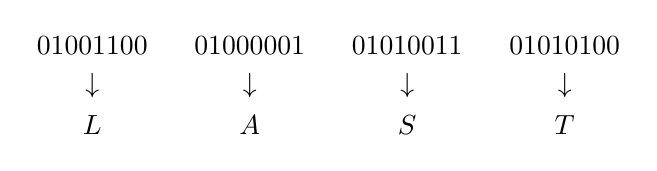
\begin{tikzpicture}
		\draw (2,2) node {$01001100$};
		\draw (4,2) node {$01000001$};
		\draw (6,2) node {$01010011$};
		\draw (8,2) node {$01010100$};
		
		\draw (2,1.5) node {$\downarrow$};
		\draw (4,1.5) node {$\downarrow$};
		\draw (6,1.5) node {$\downarrow$};
		\draw (8,1.5) node {$\downarrow$};
		
		\draw (2,1) node {$L$};
		\draw (4,1) node {$A$};
		\draw (6,1) node {$S$};
		\draw (8,1) node {$T$};
	\end{tikzpicture}
\end{figure}
The solution thus seems to be the last word on page 192 in the original bitcoin whitepaper. However, the short length of the Bitcoin whitepaper and the mentioning of the RSA algorithm in the problem description hint, that there is more to the number 192. Treating this number as the encrypted message $C$ in the RSA algorithm and using the same values for the private key $k_p$ and $N$ as in Exercise 3 gives us the solution $M = 192^{63}\;(mod\, 253) = 4$. This seems much more reasonable as reference to a page number and leads to the solution being "memory".\par 
At the end of the task we were also asked to convert the hexadecimal 4b into a decimal number. The easiest way to do this, is by first converting it into a binary number and then converting this binary number into a decimal:
	\begin{figure}[h!]
	\begin{minipage}{0.4\textwidth}
		\centering
		\begin{tikzpicture}
			\draw (2,2) node {$4$};
			\draw (4,2) node {$b$};
			
			\draw (2,1.5) node {$\downarrow$};
			\draw (4,1.5) node {$\downarrow$};
			
			\draw (2,1) node {$4$};
			\draw (4,1) node {$11$};
			
			\draw (2,.5) node {$\downarrow$};
			\draw (4,.5) node {$\downarrow$};
			
			\draw (2,0) node {$0100$};
			\draw (4,0) node {$1011$};
			
			%\draw(3,-1) node {$(01001011)_{B=2}$};
			\draw(5,1) node {$\quad \quad$ \Large{$\rightarrow$}};
		\end{tikzpicture}
	\end{minipage}
	\hfill
	\begin{minipage}{0.6\textwidth}
	\centering
	\resizebox{\linewidth}{2.045cm}{ % {width}{hight}
		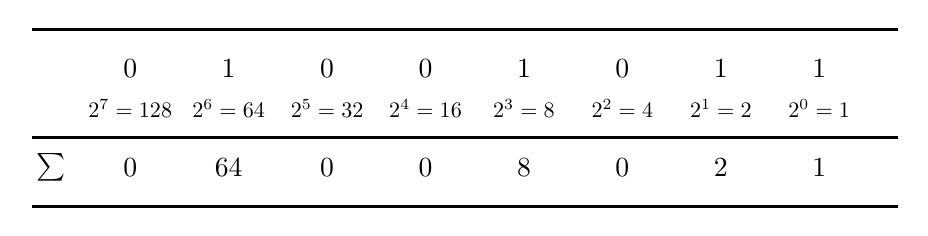
\begin{tikzpicture}[domain=0:11]
			\draw[very thick] (0,0) -- (11,0);
			\draw[very thick] (0,2.25) -- (11,2.25);
			\draw[thick] (0,.875) --(11,.875); 
			
			\draw (10,1.75) node {$1$};
			\draw (8.75,1.75) node {$1$};
			\draw (7.5,1.75) node {$0$};
			\draw (6.25,1.75) node {$1$};
			\draw (5,1.75) node {$0$};
			\draw (3.75,1.75) node {$0$};
			\draw (2.5,1.75) node {$1$};
			\draw (1.25,1.75) node {$0$};
			
			\draw (10,1.25) node [scale = 0.8] {$2^{0}=1$};
			\draw (8.75,1.25) node [scale = 0.8] {$2^{1}=2$};
			\draw (7.5,1.25) node [scale = 0.8] {$2^{2}=4$};
			\draw (6.25,1.25) node [scale = 0.8] {$2^{3}=8$};
			\draw (5,1.25) node [scale = 0.8] {$2^{4}=16$};
			\draw (3.75,1.25) node [scale = 0.8] {$2^{5}=32$};
			\draw (2.5,1.25) node [scale = 0.8] {$2^{6}=64$};
			\draw (1.25,1.25) node [scale = 0.8] {$2^{7}=128$};
			
			\draw (10,.5) node {$1$};
			\draw (8.75,.5) node {$2$};
			\draw (7.5,.5) node {$0$};
			\draw (6.25,.5) node {$8$};
			\draw (5,.5) node {$0$};
			\draw (3.75,.5) node {$0$};
			\draw (2.5,.5) node {$64$};
			\draw (1.25,.5) node {$0$};
			
			\draw (.25,.5) node {$\sum$};
			%\draw (2,-1) node {$\rightarrow \sum = 75 \rightarrow \;$ (4b)$_{B=16} = 75_{B=10}$};
		\end{tikzpicture}
	}
\end{minipage}
\end{figure}
\vspace{-0.5cm}

$ \quad \quad = (01001011)_{B=2}$ \hspace{3cm} $\rightarrow \; \sum = 75 \quad \rightarrow \;$ (4b)$_{B=16} = (75)_{B=10}$\\

To verify if you have found the correct solution you thus had to calculate the SHA256 of "\textbf{memory75}", which is the solution. Checking the SHA256 of this coincides with the hexadecimal given in the problem description.

\end{document}
